\documentclass[a4paper,12pt]{article} 

% First, we usually want to set the margins of our document. For this we use the package geometry.
\usepackage[top = 2.5cm, bottom = 2.5cm, left = 2.5cm, right = 2.5cm]{geometry} 
\usepackage[T1]{fontenc}
\usepackage[utf8]{inputenc}

% The following two packages - multirow and booktabs - are needed to create nice looking tables.
\usepackage{multirow} % Multirow is for tables with multiple rows within one cell.
\usepackage{booktabs} % For even nicer tables.

% As we usually want to include some plots (.pdf files) we need a package for that.
\usepackage{graphicx} 

% The default setting of LaTeX is to indent new paragraphs. This is useful for articles. But not really nice for homework problem sets. The following command sets the indent to 0.
\usepackage{setspace}
\setlength{\parindent}{0in}

% Package to place figures where you want them.
\usepackage{float}

% The fancyhdr package let's us create nice headers.
\usepackage{fancyhdr}

\usepackage{amsmath,amsthm,caption,amsfonts}
\usepackage[open]{bookmark}
\usepackage{minted}

\newcommand{\pard}[2]{\frac{\partial #1}{\partial #2}}


% To make our document nice we want a header and number the pages in the footer.

\pagestyle{fancy} % With this command we can customize the header style.

\fancyhf{} % This makes sure we do not have other information in our header or footer.

\lhead{\footnotesize Machine Learning (H): Assignment 4}% \lhead puts text in the top left corner. \footnotesize sets our font to a smaller size.

%\rhead works just like \lhead (you can also use \chead)
\rhead{\footnotesize Mengxuan Wu} %<---- Fill in your lastnames.

% Similar commands work for the footer (\lfoot, \cfoot and \rfoot).
% We want to put our page number in the center.
\cfoot{\footnotesize \thepage} 

\begin{document}

\thispagestyle{empty} % This command disables the header on the first page. 

\begin{tabular}{p{15.5cm}}
{\large \bf Machine Learning (H)} \\
Southern University of Science and Technology \\ Mengxuan Wu \\ 12212006 \\
\hline
\\
\end{tabular}

\vspace*{0.3cm} %add some vertical space in between the line and our title.

\begin{center}
	{\Large \bf Assignment 4}
	\vspace{2mm}

	{\bf Mengxuan Wu}
		
\end{center}  

\vspace{0.4cm}

\section*{Question 1}

The function with Lagrange multiplier is
\begin{equation*}
	C(w, \lambda) = w^T (\mathbf{m_2} - \mathbf{m_1}) + \lambda (w^T w - 1)
\end{equation*}

Take the derivative with respect to $w$ and set it to zero, we have
\begin{equation*}
	\pard{C}{w} = \mathbf{m_2} - \mathbf{m_1} + 2 \lambda w = 0
\end{equation*}

Solve the equation, we have
\begin{equation*}
	w = \frac{\mathbf{m_1} - \mathbf{m_2}}{2 \lambda}
\end{equation*}

Thus, we have $w \propto \mathbf{m_1} - \mathbf{m_2}$.

\section*{Question 2}

\begin{align*}
	J(w) &= \frac{(m_2 - m_1)^2}{s_1^2 + s_2^2} \\
	&= \frac{w^T (\mathbf{m_2} - \mathbf{m_1}) (\mathbf{m_2} - \mathbf{m_1})^T w}{\sum_{n \in C_1} (w^T (\mathbf{x_n} - \mathbf{m_1}))^2 + \sum_{n \in C_2} (w^T (\mathbf{x_n} - \mathbf{m_2}))^2} \\
	&= \frac{w^T (\mathbf{m_2} - \mathbf{m_1}) (\mathbf{m_2} - \mathbf{m_1})^T w}{w^T \left(\sum_{n \in C_1} (\mathbf{x_n} - \mathbf{m_1}) (\mathbf{x_n} - \mathbf{m_1})^T + \sum_{n \in C_2} (\mathbf{x_n} - \mathbf{m_2}) (\mathbf{x_n} - \mathbf{m_2})^T \right) w} \\
\end{align*}

Since we know
\begin{equation*}
	S_B = (\mathbf{m_2} - \mathbf{m_1}) (\mathbf{m_2} - \mathbf{m_1})^T
\end{equation*}
\begin{equation*}
	S_W = \sum_{n \in C_1} (\mathbf{x_n} - \mathbf{m_1}) (\mathbf{x_n} - \mathbf{m_1})^T + \sum_{n \in C_2} (\mathbf{x_n} - \mathbf{m_2}) (\mathbf{x_n} - \mathbf{m_2})^T
\end{equation*}

Thus, we have
\begin{equation*}
	J(w) = \frac{w^T S_B w}{w^T S_W w}
\end{equation*}

\section*{Question 3}

For each data point, we have
\begin{equation*}
	p(\{\phi, t\}) = \prod_{k=1}^K p(\phi|C_k) p(C_k) = \prod_{k=1}^K [\pi_k p(\phi|C_k)]^{t_k}
\end{equation*}

Thus, for the whole data set, we have
\begin{equation*}
	p(\{\phi_n, t_n\}) = \prod_{n=1}^N \prod_{k=1}^K [\pi_k p(\phi_n|C_k)]^{t_{nk}}
\end{equation*}

Take the log of the likelihood, we have
\begin{equation*}
	\log p(\{\phi_n, t_n\}) = \sum_{n=1}^N \sum_{k=1}^K t_{nk} \log \pi_k + t_{nk} \log p(\phi_n|C_k)
\end{equation*}

The extra constraint is
\begin{equation*}
	\sum_{k=1}^K \pi_k = 1
\end{equation*}

Thus, the Lagrange function is
\begin{equation*}
	L(\pi, \lambda) = \sum_{n=1}^N \sum_{k=1}^K t_{nk} \log \pi_k + t_{nk} \log p(\phi_n|C_k) + \lambda \left(\sum_{k=1}^K \pi_k - 1\right)
\end{equation*}

Take the derivative with respect to $\pi_k$ and set it to zero, we have
\begin{equation*}
	\pard{L}{\pi_k} = \sum_{n=1}^N \frac{t_{nk}}{\pi_k} + \lambda = 0
\end{equation*}

Solve the equation, we have
\begin{equation*}
	\pi_k = -\frac{1}{\lambda} \sum_{n=1}^N t_{nk}
\end{equation*}

Since $\sum_{k=1}^K \pi_k = 1$, we have
\begin{equation*}
	\sum_{k=1}^K \pi_k = -\frac{1}{\lambda} \sum_{n=1}^N \sum_{k=1}^K t_{nk} = 1
\end{equation*}

Thus, we have
\begin{equation*}
	\lambda = -N
\end{equation*}
\begin{equation*}
	\pi_k = \frac{1}{N} \sum_{n=1}^N t_{nk} = \frac{N_k}{N}
\end{equation*}
where $N_k$ is the number of data points in class $C_k$.

\section*{Question 4}

Taking the derivative of the sigmoid function, we have
\begin{align*}
	\pard{\sigma(a)}{a} &= \pard{}{a} \frac{1}{1 + e^{-a}} \\
	&= \frac{e^{-a}}{(1 + e^{-a})^2} \\
	&= \frac{1}{1 + e^{-a}} \frac{e^{-a}}{1 + e^{-a}} \\
	&= \sigma(a) (1 - \sigma(a))
\end{align*}

\section*{Question 5}

\begin{equation*}
	\pard{E(w)}{w} = \pard{}{w} - \sum_{n=1}^N \left[t_n \log y_n + (1 - t_n) \log (1 - y_n)\right]
\end{equation*}

Since $y_n = \sigma(w^T \phi_n)$, combining with the result in Question 4, we have
\begin{align*}
	\pard{y_n}{w} &= \pard{}{w} \sigma(w^T \phi_n) \\
	&= \sigma(w^T \phi_n) (1 - \sigma(w^T \phi_n)) \pard{}{w} w^T \phi_n \\
	&= y_n (1 - y_n) \phi_n
\end{align*}

Thus, we have
\begin{align*}
	\pard{E(w)}{w} &= - \sum_{n=1}^N \left[t_n \frac{1}{y_n} y_n (1 - y_n) \phi_n - (1 - t_n) \frac{1}{1 - y_n} y_n (1 - y_n) \phi_n\right] \\
	&= - \sum_{n=1}^N \left[t_n (1 - y_n) \phi_n - (1 - t_n) y_n \phi_n\right] \\
	&= - \sum_{n=1}^N \left[t_n - y_n\right] \phi_n \\
	&= \sum_{n=1}^N \left[y_n - t_n\right] \phi_n
\end{align*}

\newpage
\section*{Question 6}

For the first approach, we have
\begin{figure}[H]
	\centering
	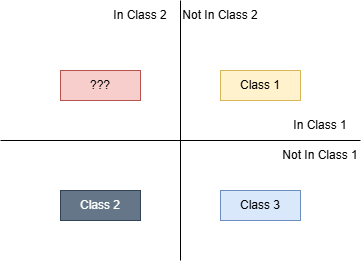
\includegraphics[width=0.9\textwidth]{figure/Question6.1.drawio.png}
\end{figure}

For the second approach, we have
\begin{figure}[H]
	\centering
	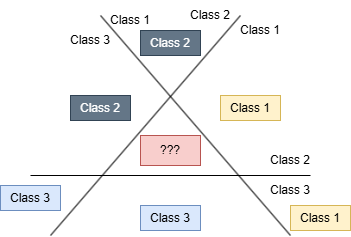
\includegraphics[width=0.9\textwidth]{figure/Question6.2.drawio.png}
\end{figure}

\section*{Question 7}

\subsection*{Convex hulls intersect $\Rightarrow$ Sets are not linearly separable}

If two convex hulls intersect, then there must be at least a point that is in both convex hulls. Let the point be $\mathbf{x}$, then we have
\begin{equation*}
	\mathbf{x} = \sum_{n=1}^{N} \alpha_n \mathbf{x}^n = \sum_{m=1}^{M} \beta_m \mathbf{z}^m
\end{equation*}
where $\alpha_n \geq 0$, $\sum_{n=1}^{N} \alpha_n = 1$, $\beta_m \geq 0$, $\sum_{m=1}^{M} \beta_m = 1$.

Suppose there exists a vector $\hat{w}$ and a scalar $w_0$ that can linearly separate the two convex hulls, then we have
\begin{equation*}
	\hat{w}^T \mathbf{x}^n + w_0 > 0 \quad \forall n
\end{equation*}
\begin{equation*}
	\hat{w}^T \mathbf{z}^m + w_0 < 0 \quad \forall m
\end{equation*}

Thus, we have
\begin{equation*}
	\hat{w}^T \mathbf{x} = \hat{w}^T \sum_{n=1}^{N} \alpha_n \mathbf{x}^n = \sum_{n=1}^{N} \alpha_n \hat{w}^T \mathbf{x}^n > 0
\end{equation*}
\begin{equation*}
	\hat{w}^T \mathbf{x} = \hat{w}^T \sum_{m=1}^{M} \beta_m \mathbf{z}^m = \sum_{m=1}^{M} \beta_m \hat{w}^T \mathbf{z}^m < 0
\end{equation*}

There is a contradiction, thus the two convex hulls cannot be linearly separated.

\subsection*{Sets are linearly separable $\Rightarrow$ Convex hulls do not intersect}

This is the contrapositive of the first part, thus it has the same truth value, which is true.

\end{document}